\onecolumn
\chapter{Veruschsaufbauten}
Im folgenden sind die verschiedenen Veruschsaufbauten mit ihren Maßen aufgelistet. Werte, die mit einem Strich versehen sind, sind gemessene Werte. Jene ohne Strich sind berechnete Werte. Die Maßstäbe sind möglichst präzise gesetzt.

\begin{figure}[!ht]
    \section{Maße der Rollebene}
    \centering
    \includegraphics[width=1\textwidth]{img/15/Maße-RollEbene.pdf}
    \caption{Gemessene Längen der Abrollebene, zudem der Berechnete Neigungswinkel und die berechnete Starthöhe.}
    \label{fig:maße_re}
\end{figure}

\begin{figure}[!ht]
    \section{Maße der LS Messung Beschelunigung}
    \centering
    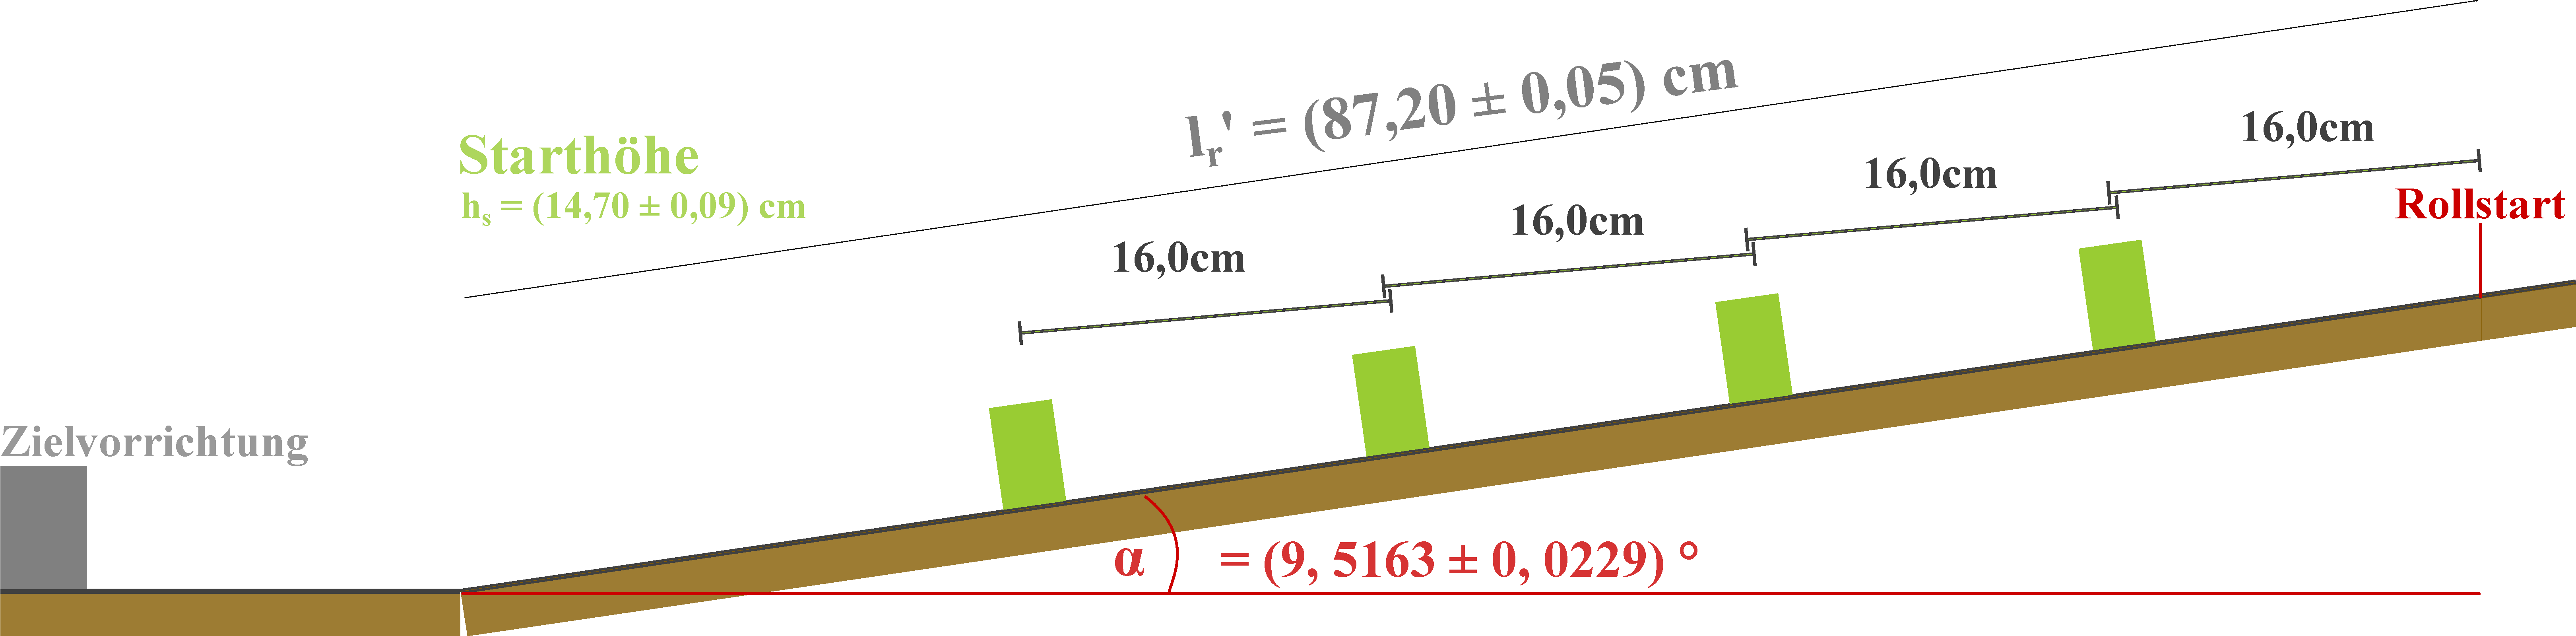
\includegraphics[width=1\textwidth]{img/15/Aufbau2.pdf}
    \caption{Gemessene Längen der Abrollebene, zudem der Berechnete Neigungswinkel und die berechnete Starthöhe.}
    \label{fig:maße_2}
\end{figure}

\begin{figure}[!ht]
    \section{Maße der LS Messung Geschwindigkeit}
    \centering
    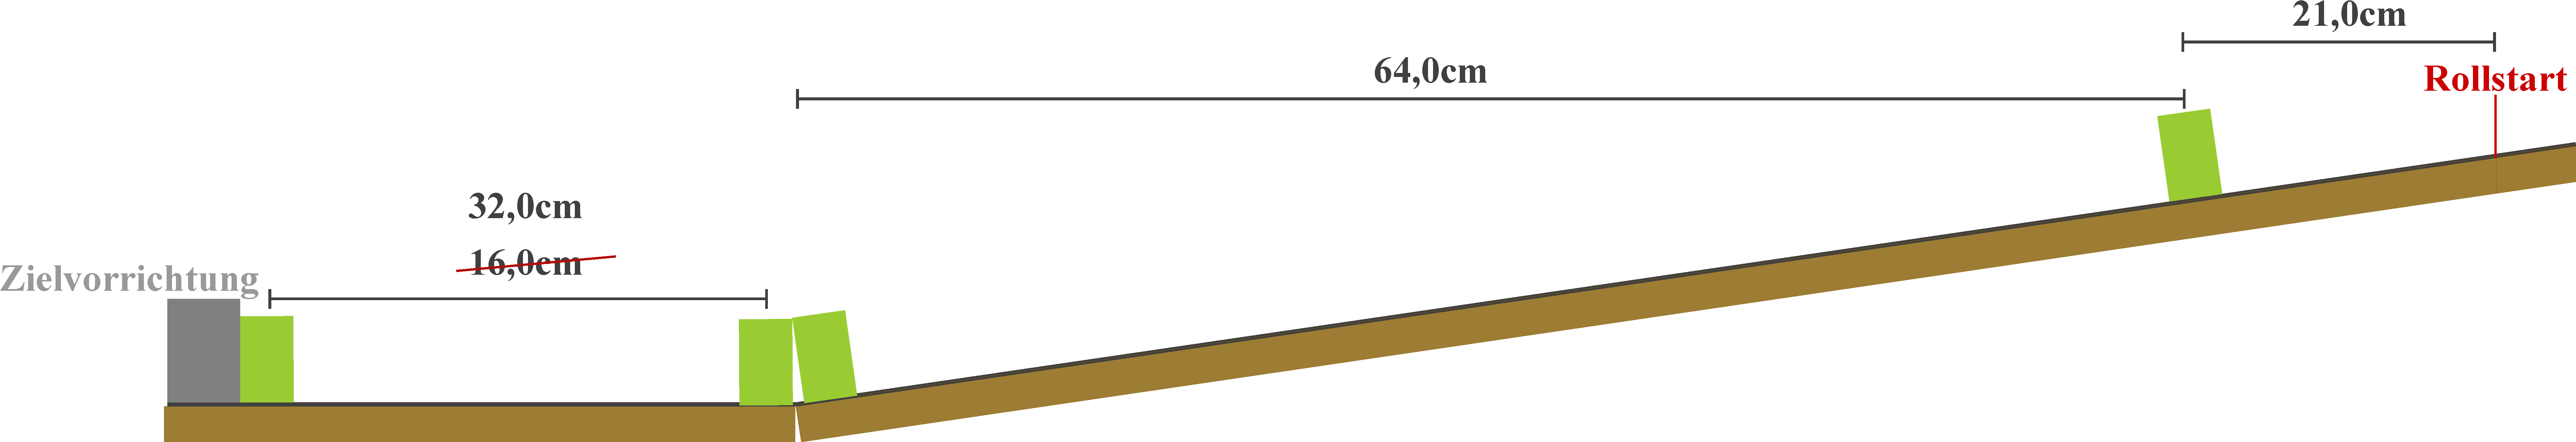
\includegraphics[width=1\textwidth]{img/15/Aufbau3.pdf}
    \caption{Gemessene Längen der Abrollebene, zudem der Berechnete Neigungswinkel und die berechnete Starthöhe.}
    \label{fig:maße_3}
\end{figure}

\begin{figure}[!ht]
    \section{Maße der Messzylinder}
    \centering
    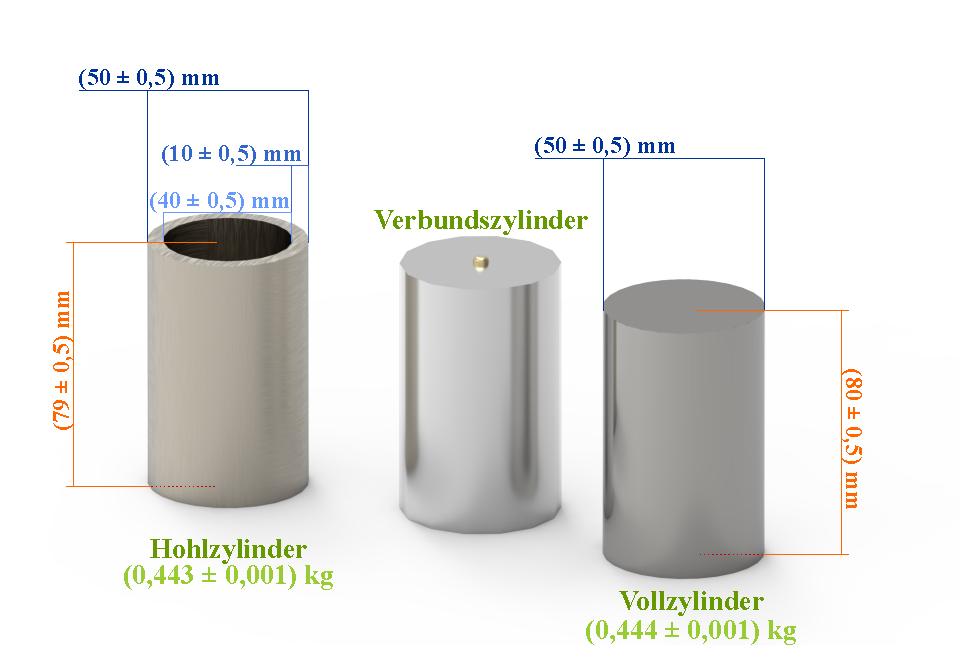
\includegraphics[width=0.85\textwidth]{img/15/Zylindermasse.pdf}
    \caption{3D-Rendering mit den vermessene Größen der Zylinder eingezeichnet (Maßstabsgetreu).}
    \label{fig:zylinder_masse}
\end{figure}
\twocolumn